%% LyX 2.0.2 created this file.  For more info, see http://www.lyx.org/.
%% Do not edit unless you really know what you are doing.
\documentclass[american]{spie}
\usepackage[T1]{fontenc}
\usepackage[latin9]{inputenc}
\usepackage[letterpaper]{geometry}
\geometry{verbose,tmargin=2.54cm,bmargin=3.17cm,lmargin=2.22cm,rmargin=2.22cm}
\setcounter{secnumdepth}{3}
\setcounter{tocdepth}{3}
\usepackage{textcomp}
\usepackage{amsmath}
\usepackage{graphicx}

\makeatletter

%%%%%%%%%%%%%%%%%%%%%%%%%%%%%% LyX specific LaTeX commands.
\newcommand{\lyxmathsym}[1]{\ifmmode\begingroup\def\b@ld{bold}
  \text{\ifx\math@version\b@ld\bfseries\fi#1}\endgroup\else#1\fi}

%% Because html converters don't know tabularnewline
\providecommand{\tabularnewline}{\\}

\makeatother

\usepackage{babel}
\begin{document}

\title{Regularized self-tuning phase demodulation for phase-shifting interferometry
with arbitrary phase shifts}


\author{Orlando Medina\supit{a}, Julio C. Estrada\supit{a}, Manuel Servin\supit{a}\skiplinehalf \supit{a}Centro de Investigaciones en �ptica, Loma del bosque 115 Col. Lomas del campestre, 37150, Le�n Guanajuato, M�xico.}\authorinfo{Further author information: E-mail: orlandomedina@cio.mx}
\maketitle
\begin{abstract}
In this work, we develop a regularization technique to demodulate
a phase-shifting interferogram sequence with arbitrary inter-frame
phase shifts. With this method, we can recover the modulating phase
and inter-frame phase shifts in the same process. As all phase-shifting
algorithms, the assumption is that the wavefront under test does not
change over time, but the introduction of phase-shifts can vary in
a non constant way. A notable characteristic of this demodulation
method is that not only can it recover the modulating phase, but it
is also capable of filtering-out large amounts of corrupting noise.
We will show numerical experimental results and comparisons with another
already published method to see the performance of the demodulation
technique developed herein.

\keywords{Interferometry, phase-shifting, phase demodulation, self-tuning method, arbitrary phase-shifts, noise filtering.}
\end{abstract}

\section{Introduction}

Nowadays, Phase Shifting Interferometry (PSI) techniques are some
of the most used techniques in optical metrology\cite{a1_OpticalTesting}.
In PSI, one obtains an small sequence of at least 3 interferograms
with a phase-shift among them\cite{a1_OpticalTesting}. To recover
the modulating phase, there are standard demodulation PSI methods,
the well known 3-, 4-, and 5-step phase-shifting algorithms. Knowing
the inter-frame phase-shifts (or temporal carrier), the standard methods
recover the 2$\pi$ modulus phase map with the minimum possible error\cite{a1_OpticalTesting,a2_F&K,a3}.
If we do not know the phase-shifts exactly, we obtain a phase map
with an unavoidable detuning error whose magnitude depends on the
number of interferograms employed and on how far we are from the actual
phase-shifts\cite{a3,a4,a5,a6}. This unfortunate case can occur when
the optical interferometer setup is uncalibrated or when perturbations
from the environment affect the interferometer\textquoteright{}s optical
path. For example, for most phase shifters, such as a piezoelectric
(PZT), there is a repeatability problem arising from hysteresis, non
linearity and temperature linear drift\cite{a5,a7}; curiously, the
first phase-shifting algorithms were self-tuning nonlinear algorithms\cite{a8,a9}.
To reduce detuning errors, other approaches propose error compensating
algorithms that basically use redundant data, such as the Schwider-Hariharan
5-step algorithm\cite{a4,a10,a11}, and more recently, the 9-step
algorithm shown in Ref. 12 has been used to do it by constructing
a wide-band frequency response of the phase-shifting algorithm. Further
methods use the Fourier transform in order to estimate the inter-frame
phase-shifts\cite{a6,a13}, and others are based on the least-squares
scheme, iteratively estimating the inter-frame phase-shifts and phase\cite{a14,a15}.
Ref. 16 presentes an approach that estimates the local temporal carrier
(the phase-shift) as the average of the phase difference between two
consecutive phase maps obtained from two realizations of the tunable
3-step algorithm. What we are going to show in this work is a regularized
self-tuning demodulation technique that obtains the analytical image
(complex interferogram) and inter-frame phase-shifts from an interferogram
sequence. Thus, we can recover the modulating phase 2$\pi$ modulus
and the inter-frame phase shifts in the same process. Here, it is
not necessary to know the inter-frame phase-shifts. These inter-frame
phase-shifts can vary arbitrarily. The main difference between the
demodulation method presented here and the ones reported in 14, 15
and 17 is that our demodulation method is based on a regularization
technique that is able to remove noise from its input and is robust
to non constant modulation variations, which is an issue that introduces
errors in the methods in works 14 and 15. Besides, we do not require
to estimate the fringe orientation, as the method in work 17.


\section{Method }

In general, an interferogram sequence with arbitrary inter-frame phase-shifts
can be modeled as 
\begin{equation}
I_{k}(x,y)=a(x,y)+b(x,y)cos(\phi(x,y)+\alpha_{k}),\; k=0,1,2,...,N-1,\label{eq:Ik}
\end{equation}
 where $I_{k}(x,y)$ is the intensity at the site $(x,y)$ of the
\emph{k}-interferogram in a sequence of $N-1$ interferograms, being
$a(x,y)$ its background illumination, $b(x,y)$ its contrast or modulation,
$\phi(x,y)$ the modulating phase under test and $\alpha_{k}$ the
phase-shift of the \emph{k}-interferogram. We can remove the background
illumination of each interferogram in the following way: 
\begin{equation}
I_{k}^{'}(x,y)=I_{k}(x,y)-[I_{k}*h](x,y),\; k=0,1,2,...,N-1,\label{eq:I'}
\end{equation}
where $h(x,y)$ is the impulse response of a low-pass filter, such
as a Gaussian or mean filter, and \textasteriskcentered{} is the convolution
operator\cite{a20}. After doing this, the new interferogram sequence
looks like 
\begin{equation}
I_{k}^{'}(x,y)=b^{'}(x,y)cos(\phi(x,y)+\alpha_{k}),\: k=0,1,2,...,N-1.\label{eq:I'2}
\end{equation}
The main idea of the regularized self-tuning demodulation method that
we show here comes from the article of Marroquin et al.\cite{a18}.
The demodulation process presented by Marroquin et al. minimizes a
nonlinear system that estimates the complex field of the first interferogram
and its local spatial frequencies. Unlike Marroquin et al. ,we estimate
the inter-frame phase-shifts from the interferogram sequence; therefore,
our demodulation method minimizes the following quadratic functional
\begin{eqnarray}
U(f,\alpha) & = & \sum_{(x,y)}(\varphi(x,y)-I_{0}^{'}(x,y))^{2}+\sum_{k=1}^{N-1}\sum_{(x,y)}[\frac{1}{2}[f(x,y)e^{i\alpha_{k}}+f^{*}(x,y)e^{-i\alpha_{k}}]-I_{k}^{'}(x,y)]^{2}\label{eq:U}\\
 &  & +\lambda\sum_{(x,y)}[||D_{x}[f(x,y)]||^{2}+||D_{y}[f(x,y)]||^{2}],\nonumber 
\end{eqnarray}
where $f=\left\{ f(x,y)=\varphi(x,y)+i\psi(x,y):(x,y)\in L\right\} $
is the complex field to find, $i=\sqrt{-1}$, and $f^{*}$ its complex
conjugated. The sums with the notation $(x,y)$ underneath run over
all valid $(x,y)$ sites in $L$ of the interferograms. Operators
$D_{x}[]$ and $D_{y}[]$ take the first order differences along the
$x$ and $y$ direction, as follows:
\begin{equation}
D_{x}[f(x,y)]=f(x,y)-f(x-1,y),
\end{equation}
\begin{equation}
D_{y}[f(x,y)]=f(x,y)-f(x,y-1).
\end{equation}
Regularization parameter $\lambda$ controls the smoothness of the
complex field\cite{a18,a19}. The first and second terms are the data
terms, and the third term is the regularization term. Our reference
is the first interferogram; therefore, we consider that its phase-shift
is $\alpha_{0}=0$. This is the reason of the first data term, which
results when $k=0$, and therefore, the second data term starts in
$k=1$. The minimization process of functional (4) leads to a robust
to noise nonlinear phase-shifting algorithm of N-steps that can recover
the modulating phase and inter-frame phase shifts. With the complex
field $\widehat{f}$ and phase-shifts $\alpha$ that minimize (4),
the modulating phase is recovered as 
\begin{equation}
\phi(x,y)=arg[\widehat{f}(x,y)]=arctan\left[\frac{\hat{\psi}(x,y)}{\widehat{\varphi}(x,y)}\right].\label{eq:fi}
\end{equation}
The minimization of functional (4) turns us to a nonlinear system
that is mathematically impossible to solve trough a direct numerical
method. The dimension problem is $m$ x $n$ x $N$, where $m$ x
$n$ is the interferogram dimension, and $N$ is the number of interferograms.
For nonlinear systems, the iterative\emph{ }steepest-descent algorithm
can converge to local minimums if its parameters are set adequately\cite{a21},
but its convergence speed turns out to be very slow in this case.
Then, we split the problem in two: the linear part and the nonlinear
part. The linear part are the equations that result by making the
partials $\frac{\partial U}{\partial\varphi(x,y)}$ and $\frac{\partial U}{\partial\psi(x,y)}$
zero for all $(x,y)\in L$. The nonlinear part are the equations that
result by making the partial $\frac{\partial U}{\partial\alpha_{k}}$
zero for $k=0,1,2,...,N-1$. Thus, to speed up the minimization process,
our iterative minimization strategy combines the Gauss-Seidel update
for the linear part and the steepest-descent update for the nonlinear
part in each iteration. Then, the iterations of our minimization strategy
are given with the following updates: 

\begin{equation}
\varphi^{n+1}(x,y)=Solve\: for\:\varphi^{n}(x,y)\: Eq.\left[\frac{\partial U(\varphi^{n}+i\psi^{n},\alpha^{n})}{\partial\varphi(x,y)}=0\right];\;\forall(x,y)\in L
\end{equation}


\begin{equation}
\psi^{n+1}(x,y)=Solve\: for\:\psi^{n}(x,y)\: Eq.\left[\frac{\partial U(\varphi^{n}+i\psi^{n},\alpha^{n})}{\partial\psi(x,y)}=0\right];\;\forall(x,y)\in L
\end{equation}


\begin{equation}
\alpha_{k}^{n+1}=\alpha_{k}^{n}-\mu\frac{\partial U(\varphi^{n}+i\psi^{n},\alpha^{n})}{\partial\alpha_{k}},\: k=0,1,2,...,N-1.
\end{equation}
Equations (8) and (9) correspond to the Gauss-Seidel update, and equation
(10) is the steepest-descent update. In the appendix at the end of
this paper, we show the explicit formulas of these equations. To see
this implementation, the reader can download the source code following
the web link of Ref. 22. Note: the provided source code of Ref. 22
is for illustration purposes, and it is no optimized as the C-language
code used for our numerical experiments.


\section{Numerical experiments and results}

To obtain the results presented here, the minimization process described
here made 1000 iterations to reach a relative convergence error of
$1.322\, x\,10^{-4}$. This relative convergence error is calculated
as $\sqrt{\sum(\alpha_{k}^{n}-\alpha_{k}^{n+1})^{2}}$, where the
sum runs over $k=1,2,3,...N\text{\textminus}1$, $\alpha_{k}^{n}$
is the \emph{k}-phase-shift estimated in the current iteration and
$\alpha_{k}^{n+1}$ is the \emph{k}-phase-shift of the next iteration.
This minimization process, coded and compiled in C-language, took
a time of 11.310 seconds for these 512 \texttimes{} 512 interferogram
frames in a computer with an 8-core CPU of 1.73GHz having 8GB of RAM
memory. Regularization parameter $\lambda$ (see Eq. (4)) was set
to $\lambda=10$, and parameter $\mu$ of the steepest-descent update
was $\mu=\frac{1.2}{512x512}$ (see Eq. (10)). Actually, choosing
$\mu=\frac{1.2}{512x512}$ is a very good parameter for the steepest-descent
update of Eq. (10), where $m$ \texttimes{} $n$ is the dimension
of the interferogram frames. In our numerical experiments, we always
start the minimization process with initial values of $f=0$, and
$\alpha_{k}=k\frac{\pi}{2}$ for $k=0,1,2...,N\text{\textminus}1$.
The interferogram sequence was generated as follows: the \emph{k}-frame
is given as $I_{k}=b(x,y)cos(\phi(x,y)+\alpha_{k})+\eta(x,y)$, being
$\eta(x,y)$ a random field of white noise with mean $\gamma=0$ and
variance $\sigma^{2}=4.84$ radians. The modulation, or contrast term
$b(x,y)$, was modeled as a parabola centered at pixel $(256,256)$
of the image frames with a dynamic range between 1 and 3. The inter-frame
phase-shifts were generated as $\alpha_{k}=\pi+0.4*\varepsilon$ ,
where $\varepsilon_{k}$ is a random scalar with a uniform distribution
between $-\pi$ and $\pi$ radians. Here, we compare our results with
the so called Advanced Iterative Algorithm (AIA) presented in Ref.
15 because this method estimates the phase and inter-frame phase-shifts
as well, but using another approach. In Table. 1
\begin{table}
\begin{centering}
\begin{tabular}{|c|c|c|}
\hline 
Steps & Proposed Method & AIA Method\tabularnewline
\hline 
\hline 
0 & 0 & 0\tabularnewline
\hline 
1 & 0.0766 & 0.0904\tabularnewline
\hline 
2 & 0.0637 & 0.7146\tabularnewline
\hline 
3 & 0.0569 & 0.7083\tabularnewline
\hline 
4 & 0.0569 & 0.5520\tabularnewline
\hline 
\end{tabular}
\par\end{centering}

\caption{This table shows the error obtained between the phase-shift estimation
and the actual phase-shift.}


\end{table}
, we show the error values of the estimated phase-shifts using our
regularized method and the estimated using the AIA method. These errors
are calculated as $|\alpha_{k}\lyxmathsym{\textminus}\widehat{\alpha}_{k}|$,
where $\hat{\alpha}_{k}$ and $\alpha_{k}$ are the values of the
estimated and actual phase-shifts for the \emph{k}-frame, respectively.
There we can see that our method estimates the inter-frame phase-shifts
with less error. On the other hand, in Fig. 1
\begin{figure}
\begin{centering}
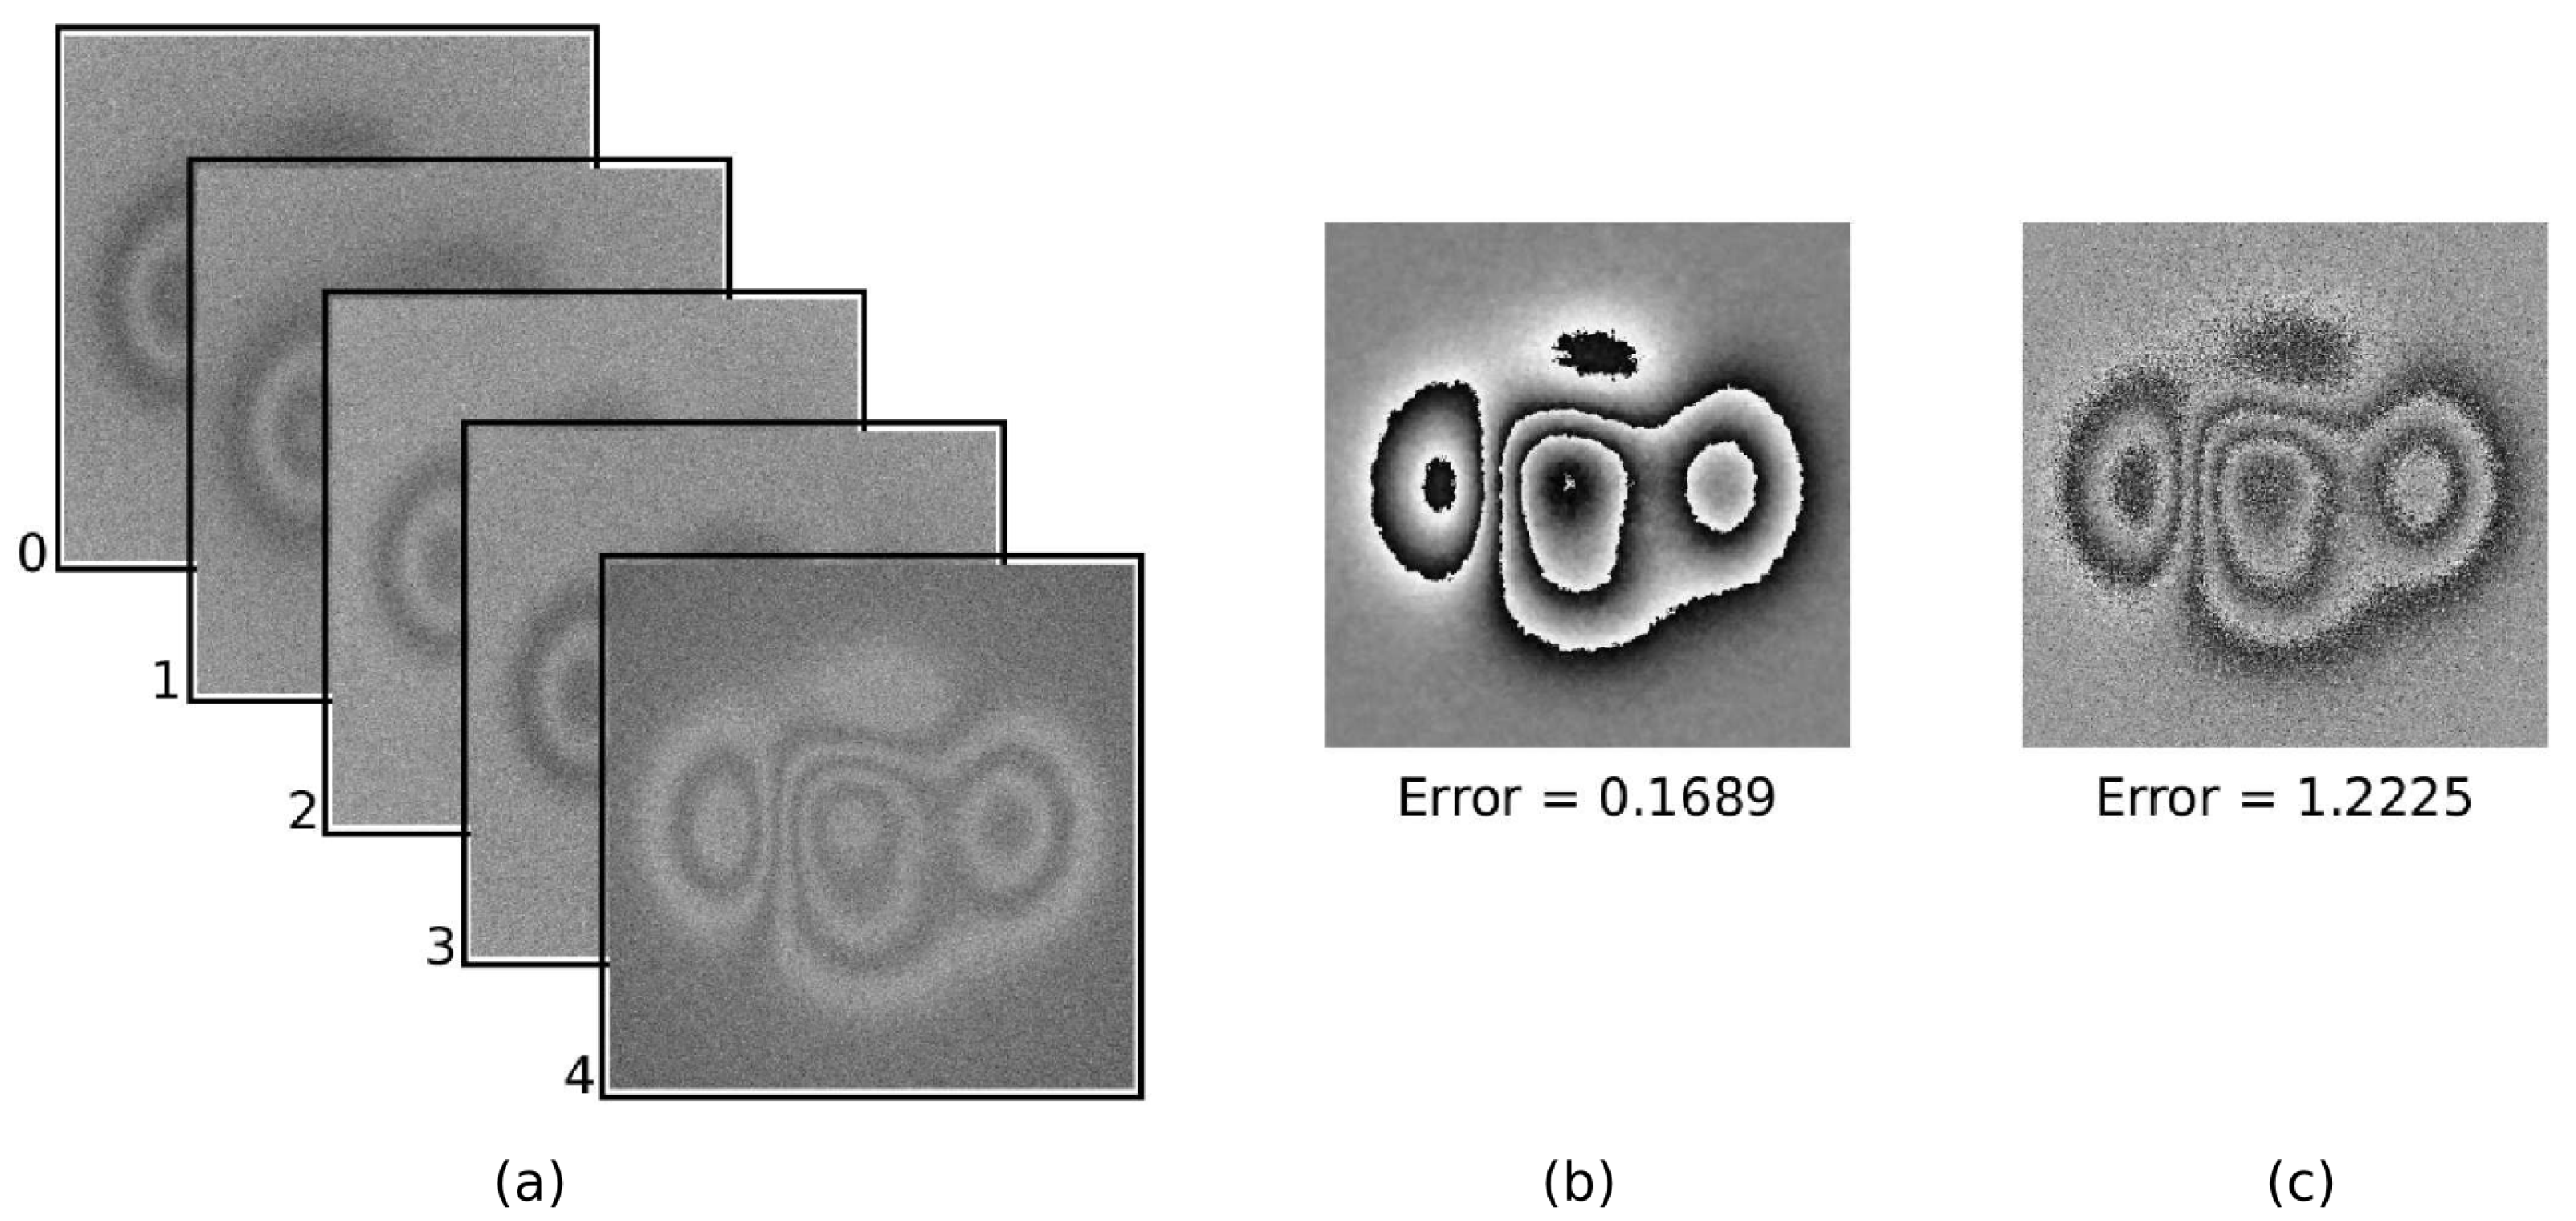
\includegraphics[scale=0.3]{Steps}
\par\end{centering}

\caption{Interferogram sequence and the recovered phase. (A) shows the recovered
phase and error using the regularized self-tuning method proposed
here. (B) shows the recovered phase and error using the AIA method{[}15{]}.
The error shown (in radians) is the standard deviation respecting
the true phase map. The interferogram frames has a size of 512 \texttimes{}
512. }


\end{figure}
 we show the interferogram sequence and the recovered phase. Fig.
1.(A) shows the recovered phase using the regularized self-tuning
demodulation method presented here, while Fig. 1.(B) shows the recovered
phase using the AIA method. We can see in this figure that our proposed
regularized self-tuning demodulation method recovers the phase with
less noise and error than the AIA method. The errors shown in Fig.
1.(A) and Fig. 1.(B) are calculated as the standard deviation of the
difference between the recovered phase map and the true phase map
used to generate the interferograms.


\section{Performance with real images}

To assess the performance of this scheme in real applications, we
present an example of real interferometric fringe pattern images.
Fig. 2.(A) shows the first interferogram of a sequence from electronic
speckle pattern interferometry (ESPI) with non-constant phase-shifts.
The ESPI fringes corresponds to ------------explicacion franjas------------.
The Fig. 2.(B) shows the real part of the field recovered by our proposed
method, as we see this real part is a version without noise of our
first input interferogram sequence. The phase map recovered by our
proposed method is shown in Fig. 2.(C). Finally estimated non-constant
phase-shifts are shown in Fig. 2.(D) 


\section{Conclusions}

We have presented a regularized self-tuning phase-shifting demodulation
method for interferogram sequences having arbitrary variations of
the inter-frame phase-shifts. This method is robust to non constant
spatial modulations. As shown in the results, our demodulation method
is able to filter-out noise, and recover the modulating phase and
the inter-frame phase-shifts with a minimum error. The demodulation
method presented here is a nonlinear demodulation method; however,
we innovate the minimization strategy by mixing the steepest-descent
update with the Gauss-Seidel update. This way, we were able to speed
up the minimization process and obtain the expected results.


\section*{APPENDIX}

The iteration updates shown in Eqs. (8), (9) and (10) are given by
taking the gradient of (4) and solving in the following way:
\begin{equation}
\varphi^{n+1}(x,y)=\frac{F_{r}(\varphi^{n}+i\psi^{n},\alpha^{n})}{H_{r}(\alpha^{n})}
\end{equation}


\begin{equation}
\psi^{n+1}(x,y)=\frac{F_{i}(\varphi^{n}+i\psi^{n},\alpha^{n})}{H_{i}(\alpha^{n})}
\end{equation}
where

\begin{eqnarray}
F_{r}(\varphi^{n}+i\psi^{n},\alpha^{n}) & = & I_{0}(x,y)+\sum_{k=1}^{N-1}[I_{k}cos(\alpha)-\psi(x,y)sin(\alpha_{k})cos(\alpha_{k})]\nonumber \\
 &  & +\lambda[\varphi(x-1,y)s(x-1,y)+\varphi(x+1,y)s(x+1,y)\\
 &  & +\varphi(x,y-1)s(x,y-1)+\varphi(x,y+1)s(x,y+1)],\nonumber 
\end{eqnarray}
\begin{eqnarray}
F_{i}(\varphi^{n}+i\psi^{n},\alpha^{n}) & = & \sum_{k=1}^{N-1}[I_{k}cos(\alpha)-\varphi(x,y)sin(\alpha_{k})cos(\alpha_{k})]\nonumber \\
 &  & +\lambda[\psi(x-1,y)s(x-1,y)+\psi(x+1,y)s(x+1,y)\\
 &  & +\psi(x,y-1)s(x,y-1)+\psi(x,y+1)s(x,y+1)],\nonumber 
\end{eqnarray}


\begin{equation}
H_{r}(\alpha)=\sum_{k=1}^{N-1}cos^{2}(\alpha_{k})+\lambda[s(x-1,y)+s(x+1,y)+s(x,y-1)+s(x,y+1)]
\end{equation}


\begin{equation}
H_{i}(\alpha)=\sum_{k=1}^{N-1}sin^{2}(\alpha_{k})+\lambda[s(x-1,y)+s(x+1,y)+s(x,y-1)+s(x,y+1)]
\end{equation}
Function $s(x_{0},y_{0})$ is an indicator function that is 1 if the
point $(x_{0},y_{0})$ is within the spatial domain of the interferograms;
otherwise, it is zero. Now, for the steepest-descent update ( phase-shifts
$\alpha$) the iteration update is:
\begin{eqnarray}
\alpha_{0}^{n+1} & = & 0\\
\alpha_{k}^{n+1} & = & \alpha_{k}^{n}-\mu\sum_{\forall(x,y)\in L}[\varphi^{n}(x,y)cos(\alpha_{k}^{n})+\psi^{n}(x,y)sin(\alpha_{k}^{n})-I_{k}(x,y)]\\
 &  & [\psi^{n}(x,y)cos(\alpha_{k}^{n})-\varphi^{n}(x,y)sin(\alpha_{k}^{n})].\nonumber 
\end{eqnarray}
\textbf{Note:} suppose that $\alpha$ has the inter-frame phase-shifts
that minimize (4). Its negative values minimize (4) as well. Then,
while minimizing (4), it is possible to obtain phase-shift values
that look different to the actual phase-shift values. This is not
a problem, since we are actually interested in the modulating phase
of the interferograms. However, it is always worth fixing the inter-frame
phase-shifts obtained in the following way:

\begin{equation}
\widehat{\alpha}_{k}=\begin{cases}
\widehat{\alpha}_{k} & if\;|\widehat{\alpha}_{k}-\widehat{\alpha}_{k-1}|<\pi\\
\widehat{\alpha}_{k}-2\pi & if\;\widehat{\alpha}_{k}-\widehat{\alpha}_{k-1}>\pi\\
\widehat{\alpha}_{k}+2\pi & if\;\widehat{\alpha}_{k}-\widehat{\alpha}_{k-1}<-\pi
\end{cases}
\end{equation}
for $k=1,2,3...N\lyxmathsym{\textminus}1$, in order to have our inter-frame
phase-shifts within the variation range($-\pi,\pi$).

\bibliographystyle{spiebib}
\nocite{*}
\bibliography{self-tuning}

\end{document}
